\documentclass[onecolumn, draftclsnofoot,10pt, compsoc]{IEEEtran}
\usepackage{graphicx}
\usepackage{url}
\usepackage{setspace}
\usepackage[final]{pdfpages}
\usepackage{tabularx}
\usepackage{geometry}
\geometry{textheight=9.5in, textwidth=7in}

% 1. Fill in these details
\def \CapstoneTeamName{		Malsano}
\def \CapstoneTeamNumber{		72}
\def \GroupMemberOne{			Brandon Jolly}
\def \GroupMemberTwo{			Katherine Jeffrey}
\def \GroupMemberThree{			Bradford Wong}
\def \CapstoneProjectName{		App to Support Field Diagnostics in Veterinary Medicine}
\def \CapstoneSponsorCompany{	Oregon Veterinary Diagnostic Laboratory}
\def \CapstoneSponsorPerson{		Dr. Christiane Loehr}

% 2. Uncomment the appropriate line below so that the document type works
\def \DocType{		%Problem Statement
				Requirements Document
				%Technology Review
				%Design Document
				%Progress Report
				}
			
\newcommand{\NameSigPair}[1]{\par
\makebox[2.75in][r]{#1} \hfil 	\makebox[3.25in]{\makebox[2.25in]{\hrulefill} \hfill		\makebox[.75in]{\hrulefill}}
\par\vspace{-12pt} \textit{\tiny\noindent
\makebox[2.75in]{} \hfil		\makebox[3.25in]{\makebox[2.25in][r]{Signature} \hfill	\makebox[.75in][r]{Date}}}}
%3. If the document is not to be signed, uncomment the RENEWcommand below
%\renewcommand{\NameSigPair}[1]{#1}

%%%%%%%%%%%%%%%%%%%%%%%%%%%%%%%%%%%%%%%
\begin{document}
\begin{titlepage}
    \pagenumbering{gobble}
    \begin{singlespace}
    	
\includegraphics[height=4cm]{coe_v_spot1}
        \hfill 
        % 4. If you have a logo, use this includegraphics command to put it on the coversheet.
        %\includegraphics[height=4cm]{CompanyLogo}   
        \par\vspace{.2in}
        \centering
        \scshape{
            \huge CS Capstone \DocType \par
            {\large\today}\par
            \vspace{.5in}
            \textbf{\Huge\CapstoneProjectName}\par
            \vfill
            {\large Prepared for}\par
            \Huge \CapstoneSponsorCompany\par
            \vspace{5pt}
            {\Large\NameSigPair{\CapstoneSponsorPerson}\par}
            {\large Prepared by }\par
            Group\CapstoneTeamNumber\par
            % 5. comment out the line below this one if you do not wish to name your team
           \CapstoneTeamName\par 
            \vspace{5pt}
            {\Large
                \NameSigPair{\GroupMemberOne}\par
                \NameSigPair{\GroupMemberTwo}\par
                \NameSigPair{\GroupMemberThree}\par
            }
            \vspace{20pt}
        }
        \begin{abstract}
        % 6. Fill in your abstract    
Currently, there are many difficulties for veterinary pathologists trying to perform remote diagnostics. There are not any effective ways for people out in the field collecting samples to communicate with specialized experts located in laboratories. As a result, this project will involve creating an Android mobile application that will be used as a bridge to connect the field personnel with the veterinary pathologists in laboratories. With this mobile application, the field personnel will be able to take pictures of the individual that is being analyzed and then send the pictures along with other data such as the patient, location, and time to a pathologist. The pathologist will then be able to use the provided information to perform a necropsy and send feedback to the field personnel. This project is intended to support remote field diagnostics in veterinary medicine.
        \end{abstract}     
    \end{singlespace}
\end{titlepage}
\newpage
\pagenumbering{arabic}
\tableofcontents
% 7. uncomment this (if applicable). Consider adding a page break.
%\listoffigures
%\listoftables
\clearpage

\section{Change Log}

% table 1
\begin{table}[!hbt]
\begin{tabularx}{\textwidth}{|>{\setlength\hsize{.6\hsize}\setlength\linewidth{\hsize}}X|>{\setlength\hsize{1.6\hsize}\setlength\linewidth{\hsize}}X|>{\setlength\hsize{.8\hsize}\setlength\linewidth{\hsize}}X|}
\hline

\hline
Section & Original & New \\
\hline
% col 1
System Functions
&
% col 2
\begin{itemize}

\item Can create field reports that can contain pictures and text information such as date, location, and patient

\item When viewing a report, a user can write messages that will be sent to the other users involved in the report

\item Take pictures using Android device's camera

\item Can write additional text details using drop-down menus in the application 

\item When connected to the internet, the user who created the report can send it to another user

\item When not connected to the internet, the application will send the report as soon as a connection is established

\item Sending a report automatically updates the MySQL database

\item The MySQL database will have a web API Interface

\item A SQLite database for native storage on the phone

\item Both databases will be expandable and searchable

\item Only users with the proper credentials can use the application

\item Only the users who created and received the report can view the report

\item Stretch Goal: Provide instant feedback on image quality for each picture taken

\end{itemize}
&
% col 3
\begin{itemize}
    \item Now uses the word "submission" instead of "report".
    \item Now any user can use the application, but only users with proper credentials can send a submission through the application. 
\end{itemize}\\

\hline

% col 1
Functional Requirements
&
% col 2

When field personnel need to send reports to the lab, they can fill out a form on the app which will have menus and prompts as well as a quota for images and text entry.
\newline
The app needs to receive messages and feedback about reports from people in the lab. 
They might need to request more information or give instructions regarding next steps in the diagnostic process. 
The app will need to ensure all needed information has been included in each report to minimize requests for additional or forgotten information. 
\newline
Users will need to log in to the app to access stored information and to attach their credentials to any reports they send. This will give them permission to see previous reports and messages sent to them from the lab. 
They should be able to log out though the menu or settings screen. 
\newline 
Users in the lab will be able to log into the database and search its contents for past reports. They will be doing this using a web interface to allow multiple user to access the database without having to search using SQL. Through this web interface, users will be add comments to reports and then send them back to the user. 
\newline
The app needs to receive messages and feedback about reports from people in the lab. 
&
% col 3
\begin{itemize}
    \item Now uses the word "submission" instead of "report".
    \item Clarified that the website is a stretch goal.
\end{itemize}\\

\hline
\end{tabularx}
\end{table}

\clearpage
% table 2

\begin{table}
\begin{tabularx}{\textwidth}{|>{\setlength\hsize{.6\hsize}\setlength\linewidth{\hsize}}X|>{\setlength\hsize{1.6\hsize}\setlength\linewidth{\hsize}}X|>{\setlength\hsize{.8\hsize}\setlength\linewidth{\hsize}}X|}
\hline

\hline
Section & Original & New \\
\hline
% col 1
User Characteristics
&
% col 2
This Android application will be used by staff members and clients of the Oregon Veterinary Diagnostics Laboratory. 
There will be people out in the field who are using the application to create and share reports. 
In addition, there will be users in the laboratory who will use the application to view reports and send feedback to the field personnel.
&
% col 3
\begin{itemize}
    \item Now uses the word "submission" instead of "report".
\end{itemize}\\

\hline

% col 1
User Interface
&
% col 2
Users will need to log in to the app to access stored information and to attach their credentials to any reports they send. 
This will give them permission to see previous reports and messages sent to them from the lab. They should be able to log out though the menu or settings screen. 
When field personnel need to send reports to the lab they can fill out a form on the app which will have menus and prompts as well as a quota for images and text entry.
&
% col 3
\begin{itemize}
    \item Now uses the word "submission" instead of "report".
\end{itemize}\\

\hline

% col 1
Software Interfaces
&
% col 2
Each report will be assigned a case number so it can be easily found again by querying the database from the app or the interface in the lab. 
The lab interface is yet to be determined. 
The app could send the field reports and the lab could review the reports using  a web interface, but that might be out of the scope of the project and is a stretch goal. 
&
% col 3
\begin{itemize}
    \item Now uses the word "submission" instead of "report".
    \item Clarified that the web interface is a stretch goal.
\end{itemize}\\

\hline

% col 1
Information Management
&
% col 2
Users will need to log in to the app to access stored information and to attach their credentials to any reports they send. 
This will give them permission to see previous reports and messages sent to them from the lab. 
&
% col 3
\begin{itemize}
    \item Now uses the word "submission" instead of "report".
    \item Clarified that the web interface is a stretch goal.
\end{itemize}\\

\hline

\end{tabularx}
\end{table}


% 8. now you write!
% Bradford is writing the introduction sections
\section{Introduction}
\subsection{System Purpose}
This mobile application is intended to serve as a means of communication between personnel in the field and pathologists in the laboratory. 
Its purpose is to improve a team's ability to perform remote diagnostics by providing a convenient way for teams to communicate information.

\subsection{System Overview}


\subsubsection{System Context}
The Oregon Veterinary Diagnostic Laboratory (OVDL) wants to create an efficient way for field personnel and lab staff to communicate for remote diagnostics. 
A lack of communication can make remote diagnostics difficult because the pathologists in the laboratories can't analyze the sample and make decisions about sample processing until the sample is back in the laboratory. 
This can prove problematic if the pathologist decides that further action is needed. 
For example, they may decide that they require additional samples and data, but the field personnel may not still be in the field or the original specimen may no longer be available when this decision is made.

\subsubsection{System Functions}

\begin{itemize}

\item Can create field submissions that can contain pictures and text information such as date, location, and patient

\item When viewing a report, a user can write messages that will be sent to the other users involved in the report

\item Take pictures using Android device's camera

\item Can write additional text details using drop-down menus in the application 

\item When connected to the internet, the user who created the report can send it to another user

\item When not connected to the internet, the application will send the report as soon as a connection is established

\item Sending a report automatically updates the MySQL database

\item The MySQL database will be able to use a web API

\item A SQLite database for native storage on the phone

\item Both databases will be expandable and searchable

\item Only users with the proper credentials can send submissions through the application

\item Only the users who created and received the report can view the report

\item Stretch Goal: Provide instant feedback on image quality for each picture taken

\end{itemize}

\subsubsection{User Characteristics}
This Android application will be used by staff members and clients of the Oregon Veterinary Diagnostics Laboratory. 
There will be people out in the field who are using the application to create and share submissions. 
In addition, there will be users in the laboratory who will use the application to view submissions and send feedback to the field personnel.

\subsection{Definitions}
\begin{table}[ht]
\caption{Definitions}
\centering
\begin{tabular}{c|c}
\hline
    Term  &  Definition\\
    \hline
    \hline
    Necropsy   &   Autopsies of non-human species\\
    \hline
    Pathology    &   The study of the causes and effects of diseases, especially the branch of medicine that deals with \\
    & the laboratory examination of samples of body tissue for diagnostic or forensic purposes\\
    \hline
\end{tabular}
\end{table}

%Katherine is writing the Requirements Section
\section{Requirements}
\subsection{Functional Requirements}
The OVDL wants a native Android mobile application that collects field data and images, stores the information on a native SQLite database, sends them to the lab's MySQL database, and gets real time feedback from the lab. 
When field personnel need to send reports to the lab, they can fill out a form on the app which will have menus and prompts as well as a quota for images and text entry.
\newline
The app needs to receive messages and feedback about submissions from people in the lab. 
They might need to request more information or give instructions regarding next steps in the diagnostic process. 
The app will need to ensure all needed information has been included in each report to minimize requests for additional or forgotten information. 
\newline
Users will need to log in to the app to access stored information and to attach their credentials to any submissions they send. This will give them permission to see previous submissions and messages sent to them from the lab. 
They should be able to log out though the menu or settings screen. 
\newline 
Users in the lab will be able to log into the database and search its contents for past submissions. They will be doing this using a web interface (stretch goal) to allow multiple user to access the database without having to search using SQL. Through this web interface, users will be add comments to submissions and then send them back to the user. 

\subsection{Usability Requirements}
A stretch goal for the app is having a feature that analyzes the images taken using the phone's built-in camera and gives the user feedback on image quality. 
It should only send images that are well lit, don’t have shadows or reflections, and clearly show the subject. 
If there is time we will try to implement it because it would be beneficial for the client. 

\subsection{Performance Requirements}
Some of the remote locations might not have a stable internet or cellular connection so the data will need to be stored until a connection can be established. Otherwise the data is stored locally on the app 

% Katherine is writing the interfaces sections
\subsection{Interfaces}
\subsubsection{User Interface}
The User Interface will be the Android app which should be easy to navigate for a user with only a basic knowledge of the app's functions. 
\newline
Users will need to log in to the app to access stored information and to attach their credentials to any submission they send. 
This will give them permission to see previous submissions and messages sent to them from the lab. They should be able to log out though the menu or settings screen. 
When field personnel need to send submissions to the lab, they can fill out a form on the app which will have menus and prompts as well as a quota for images and text entry.

\subsubsection{Software Interfaces}
A SQLite database must be able to store data and images from field users.
The lab will review these images be using API which is connected to a MySQL Server. 
Each report will be assigned a case number so it can be easily found again by querying the database from the app or the interface in the lab. 
The lab interface is yet to be determined. 
The app could send the field reports and the lab could review the reports using  a web interface, but that is a stretch goal. 

\subsection{System Modes and States}
\subsubsection{Network Connection}
Some of the remote locations might not have a stable internet or cellular connection so the data will need to be stored until a connection can be established. Once the connection is made the data should be uploaded and the lab personnel should be alerted. 

\subsubsection{Database Synchronization}
The app must work with and without an internet connection and be able to store data until an internet connection is made so the data can be sent to the database. 
An optional feature is allowing the user to decide if they want the data sent automatically when the phone connects to the internet or if they want to manually send the data once they find an internet connection.

% Katherine is writing the System Security Sections 
\subsection{System Security}
The application must adhere to the OVDL's information security needs and keep track of user’s account permissions. 

\subsubsection{Information Management}
The field personnel should only be able to access the data they gathered and the information sent to them by the lab, not data gathered by other field personnel. 
There is a hierarchy of permissions for people working in the lab as well and they must only have access to the data they are allowed to see. 
Users will need to log in to the app to access stored information and to attach their credentials to any submissions they send. 
This will give them permission to see previous submissions and messages sent to them from the lab. 
They should be able to log out though the menu or settings screen.

\subsubsection{Policies and Regulations}
We must get permission before using any of OSU's logos or images. 


\section{Verification}
\subsection{Debugging}
The app's code will be consistently debugged by Android Studio's debugger.

\subsection{Field Tests}
The delivered app should be able to collect the data and images, send them to the lab through a database, and receive messages from the lab. 
It will need to pass a field test to prove it works and all the features are correctly implemented. 

\section{Appendices}
\subsection{Assumptions and Dependencies}
\begin{itemize}
\item We are assuming users will be English speakers and have some experience using Android phones. 
\end{itemize}

\subsection{Acronyms and Abbreviations}
\begin{itemize}
\item OVDL - Oregon Veterinary Diagnostic Laboratory
\item OSU - Oregon State University 
\end{itemize}

\clearpage
\section{Gantt Chart}
\begin{figure}[htp] \centering{
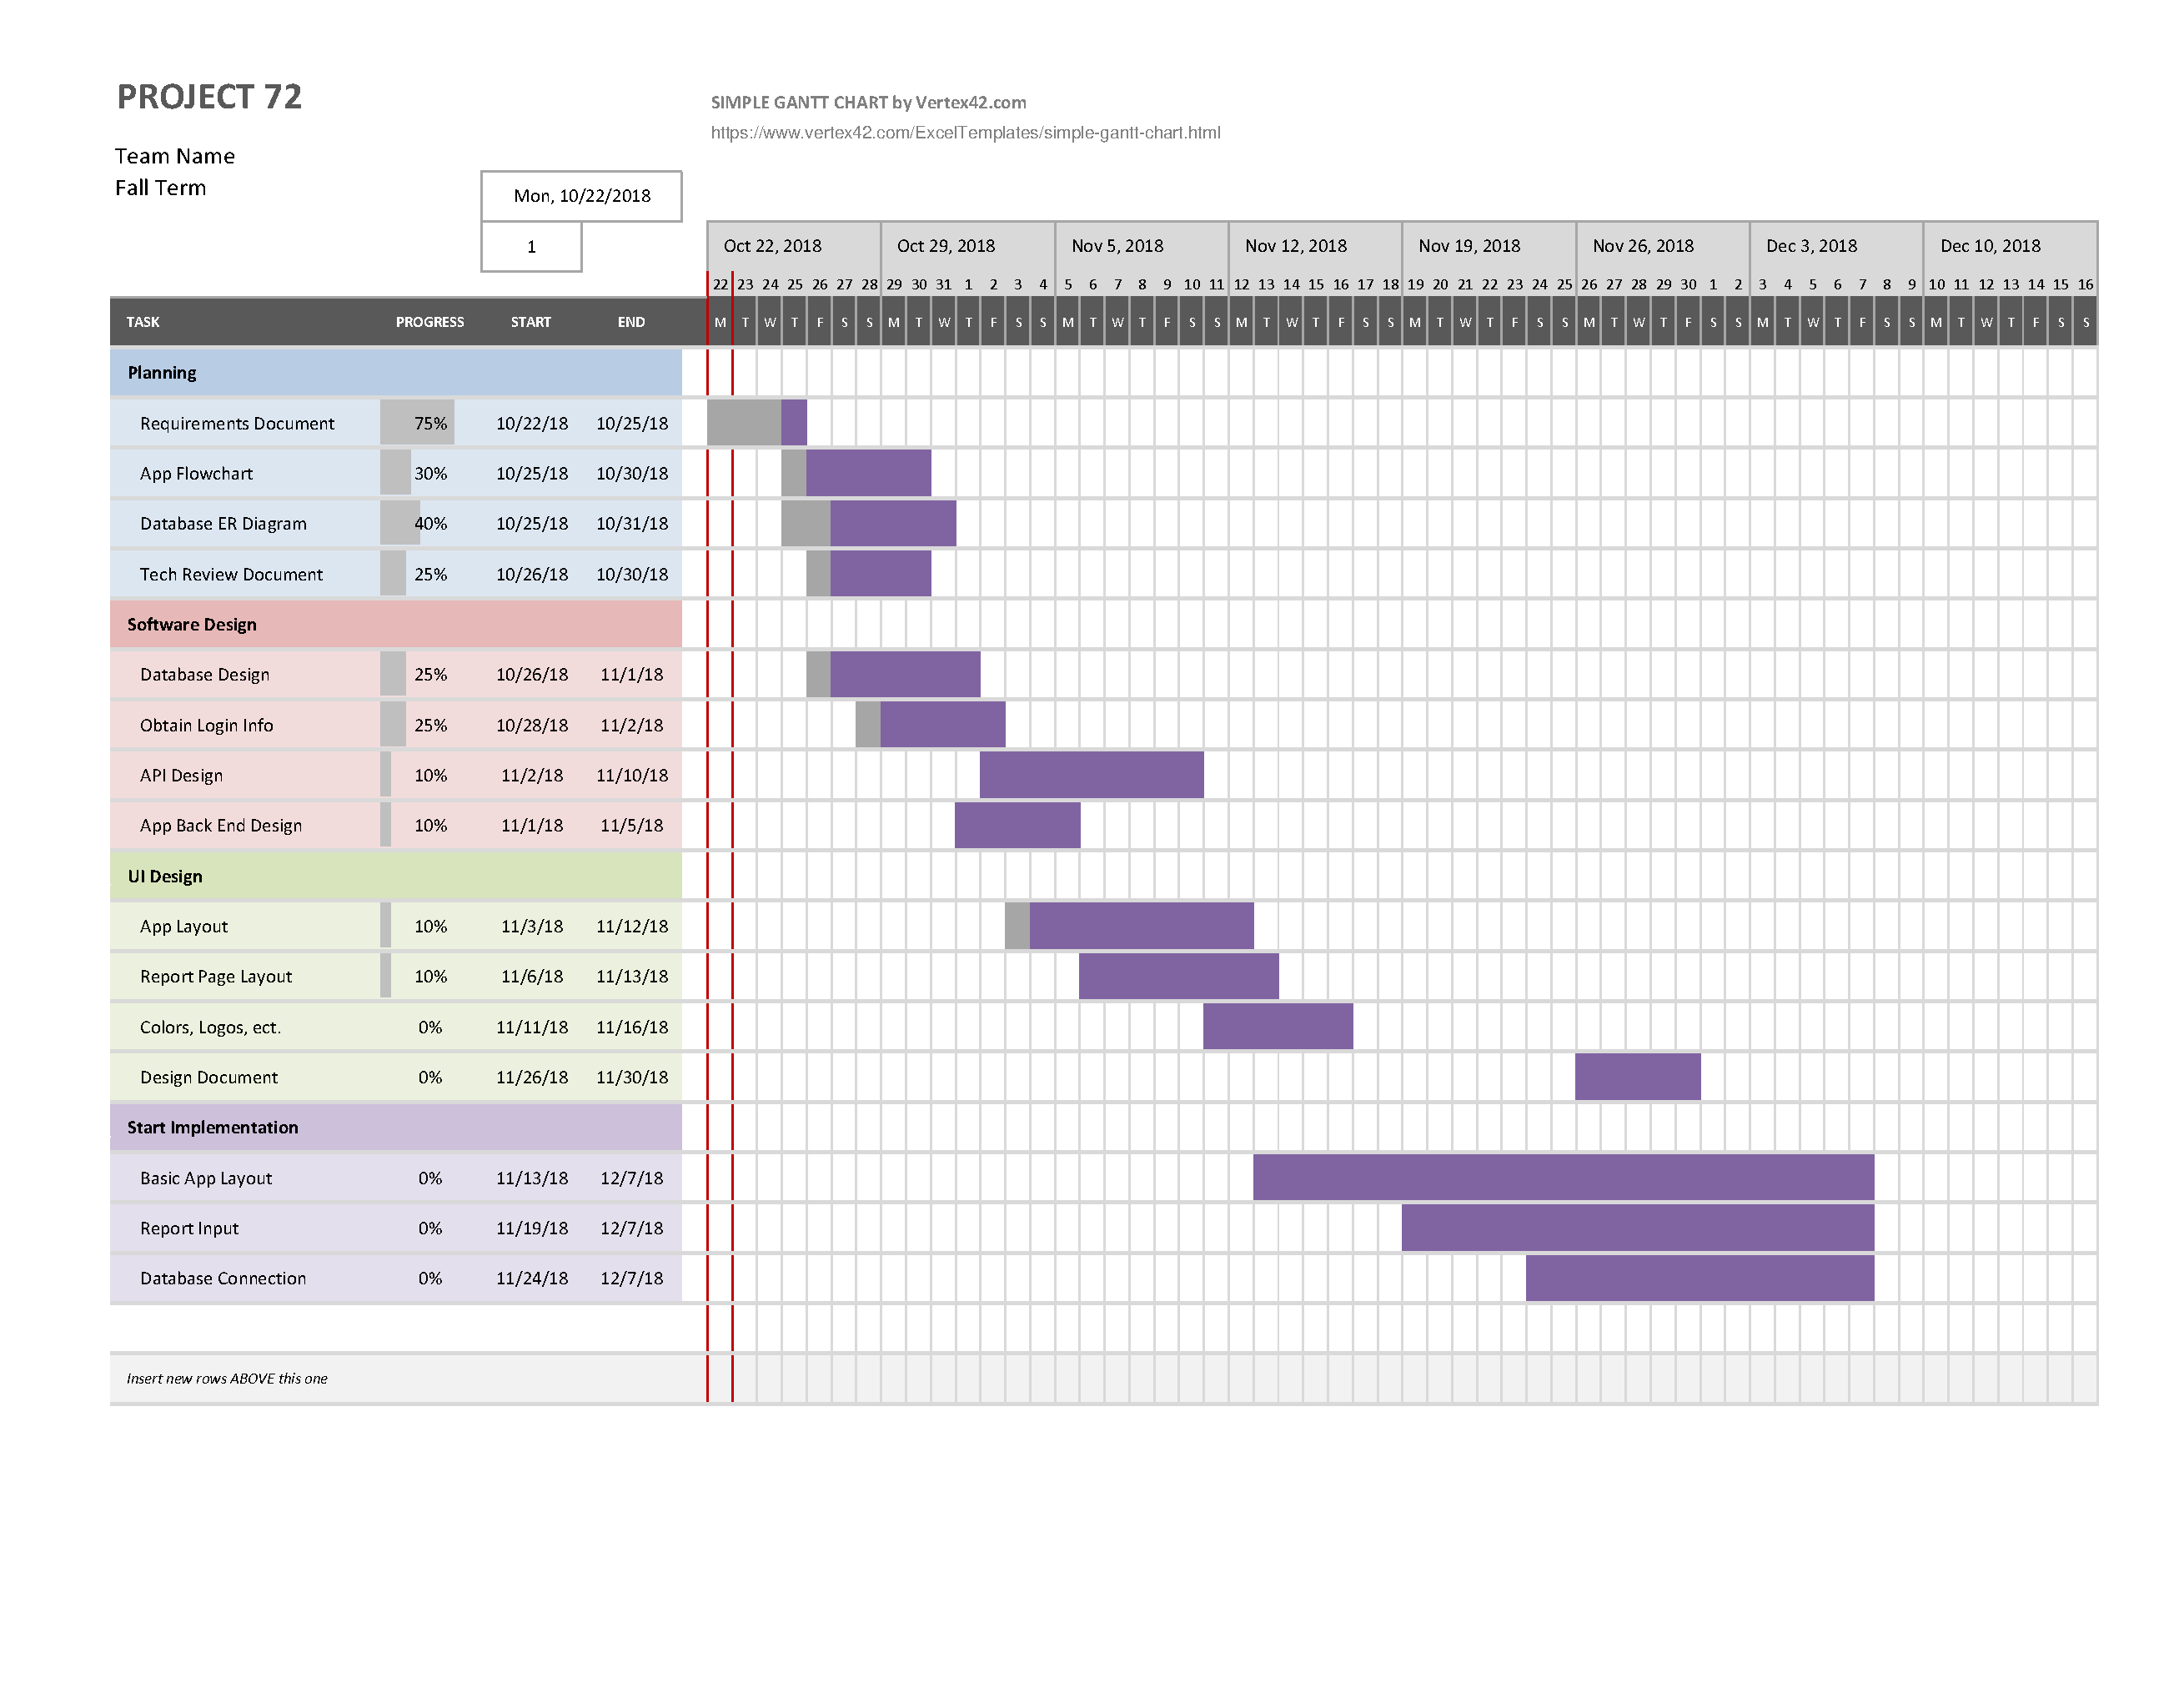
\includegraphics[scale=.45, angle=90]{GanttChart1.pdf}
}
\caption{Fall Term 2018}
\end{figure}

%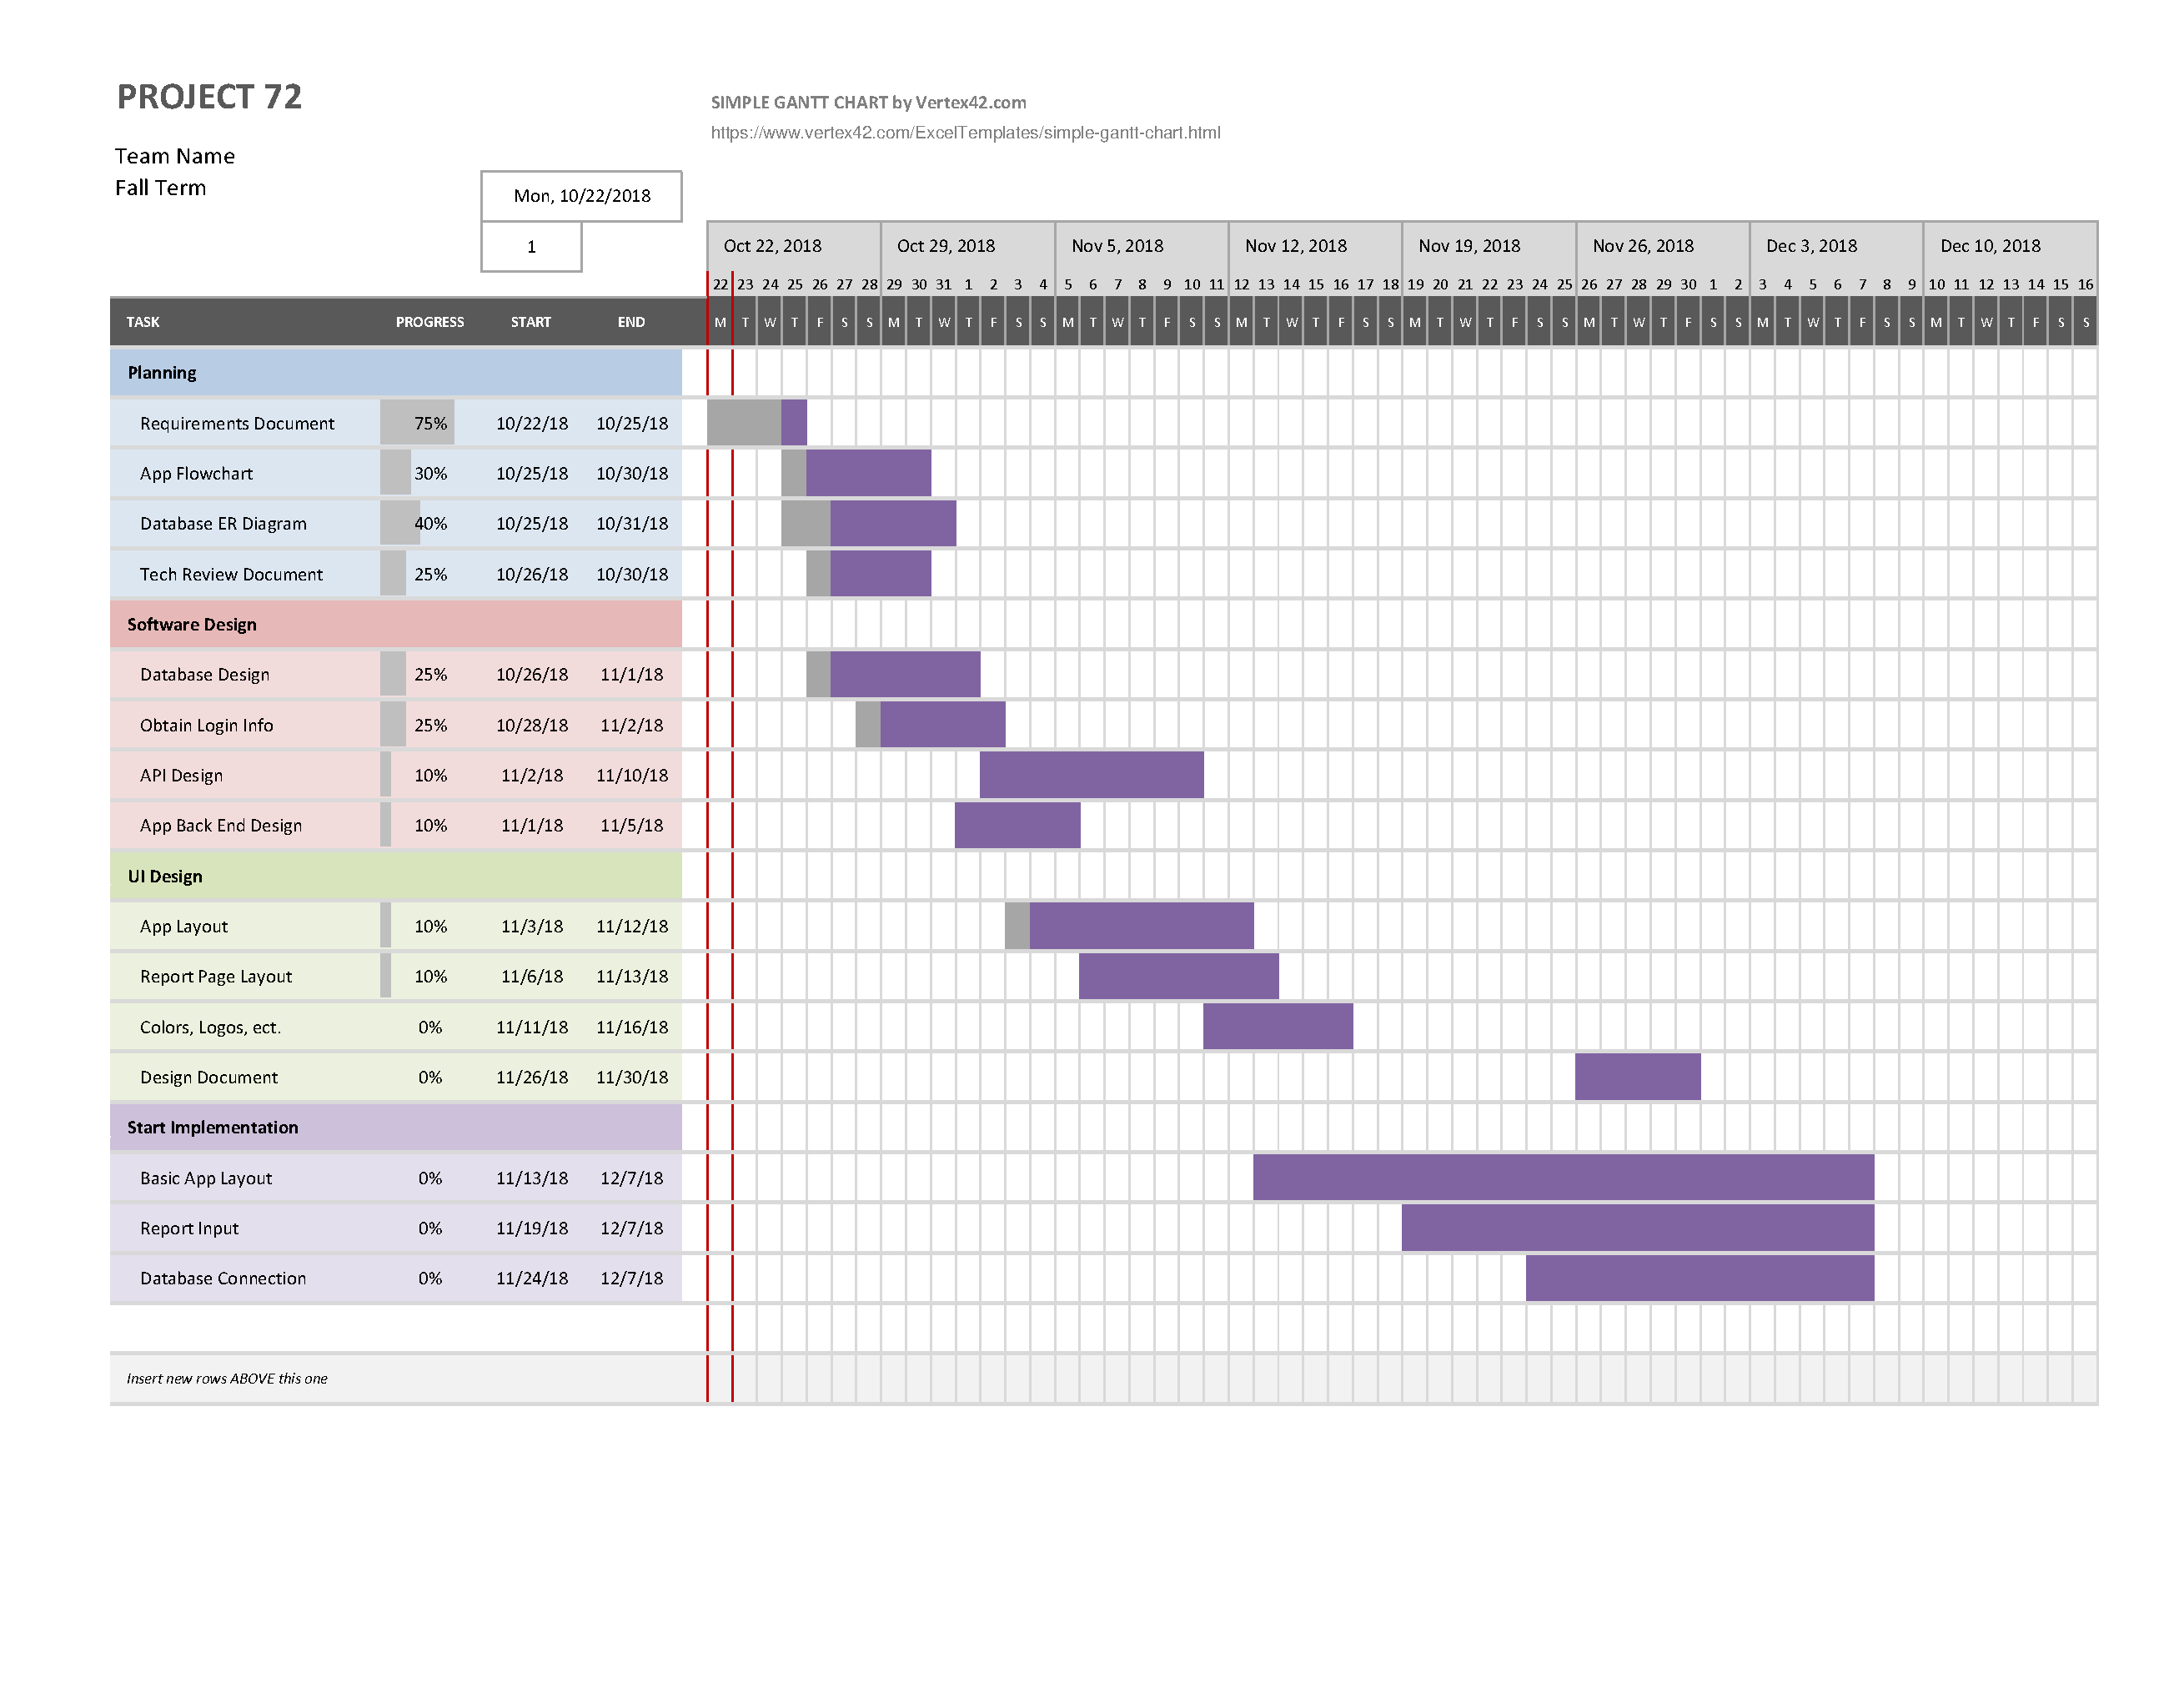
\includepdf[pages=-, angle=90, scale=.8, pagecommand={}]{GanttChart1.pdf}
 
\end{document}








